\chapter{Óptica geométrica: raios, reflexão, refração}\label{ch:b1:rays-reflection-refraction}

Um canudo dentro de um copo d'água parece quebrado na superfície; quem
nada e olha para cima do fundo de uma piscina vê o céu inteiro
comprimido num disco luminoso, cercado por um espelho do fundo; uma fibra
de vidro fina como um fio de cabelo leva uma ligação telefônica através de
um oceano com menos perda do que um fio de cobre sofre ao atravessar uma
rua. Três leis --- a luz caminha em linha reta, reflete-se com ângulos
iguais, desvia-se segundo a regra de Snell --- explicam tudo isso; este
capítulo as enuncia com precisão, marca onde deixam de valer e as põe
para trabalhar.

\begin{omfigure}
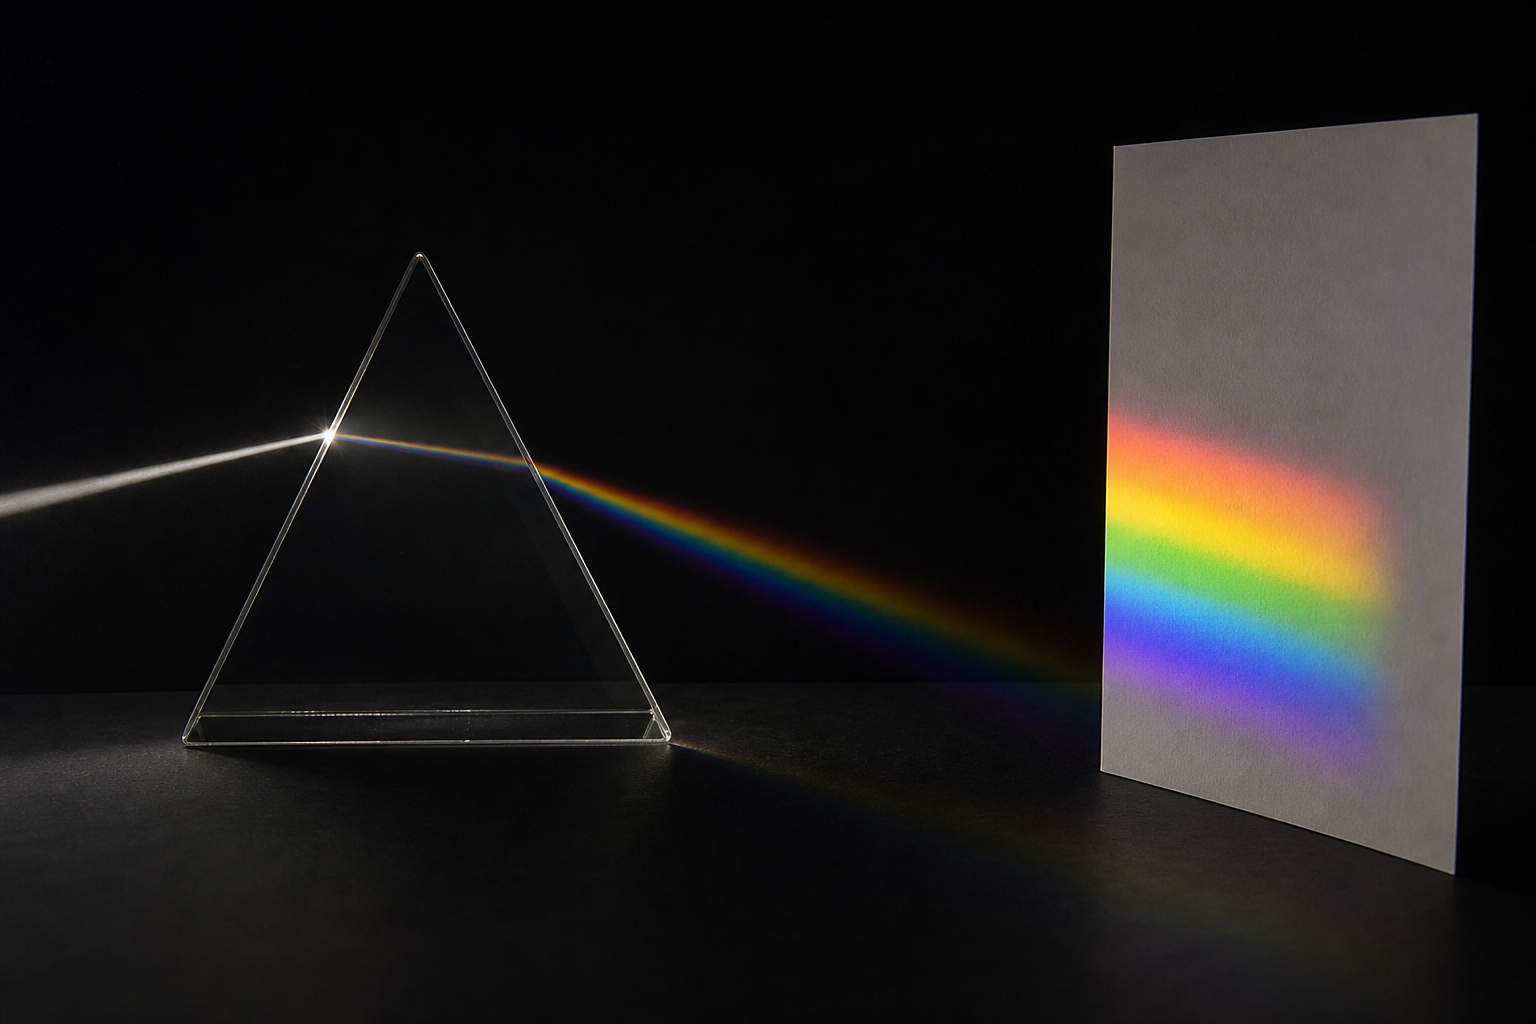
\includegraphics[width=0.58\linewidth]{images/book3/ai/b3-02-prism-dispersion-v2.png}

{\small Um prisma desvia um feixe branco em direção à sua base e o espalha: o índice do vidro depende do comprimento de onda, e o violeta é o mais desviado.}
\end{omfigure}

\section{O modelo da óptica geométrica}

\begin{definition}[Raio de luz; meio homogêneo]\label{def:b1:rays-reflection-refraction:ray}
\index{raio de luz}\index{óptica geométrica}\index{meio homogêneo}
No modelo da \emph{óptica geométrica}, a luz se propaga ao longo de
\emph{raios de luz}: curvas orientadas que são retas num meio
\emph{homogêneo} (mesmas propriedades em todos os pontos) e que
transportam energia independentemente umas das outras. Um feixe é um
conjunto de raios; uma fonte pontual emite raios em todas as direções.
\end{definition}

\begin{definition}[Índice de refração]\label{def:b1:rays-reflection-refraction:index}
\index{índice de refração}\index{meio transparente}
Um meio \emph{transparente} deixa a luz passar; nele a luz se propaga com
velocidade $v < c$. Seu \emph{índice de refração} é
\[
n = \frac{c}{v} \geq 1 .
\]
Vácuo: $n = 1$; ar: $1.0003$; água: $1.33$; vidro comum: $1.5$
a $1.6$; diamante: $2.42$. Uma onda de frequência $\nu$ conserva a sua
frequência ao entrar num meio, de modo que o seu comprimento de onda encolhe de $\lambda_0 =
c/\nu$ no vácuo para $\lambda = \lambda_0/n$.
\end{definition}

\begin{remark}[Dispersão]\label{rem:b1:rays-reflection-refraction:dispersion}
\index{dispersão (óptica)}\index{lei de Cauchy}
Na matéria o índice depende ligeiramente do comprimento de onda --- o meio é
\emph{dispersivo}. Para o vidro no visível, a lei empírica de Cauchy
$n(\lambda) = A + B/\lambda^2$ ajusta bem: $n$ é maior para o azul do que para o
vermelho, por cerca de $0.01$ a $0.02$. O prisma e o arco-íris, no fim
deste capítulo, vivem dessa diferença.
\end{remark}

\begin{remark}[Limites do modelo]\label{rem:b1:rays-reflection-refraction:limits}
A luz é uma onda, e uma onda que atravessa uma abertura de largura $a$
se espalha por um ângulo da ordem de $\lambda/a$ (difração,
\cref{ch:b1:wave-propagation}). Os raios são uma boa descrição enquanto
toda abertura, lente e obstáculo for muito maior que o comprimento de onda
(\qty{0.4}{} a \qty{0.8}{\micro m} para a luz visível): um furo de \qty{1}{mm}
espalha um feixe por $10^{-3}$ radianos, desprezível numa bancada; um
furo de \qty{1}{\micro m} o espalha por todo o semiespaço, e nenhuma imagem
de raios sobrevive. O \omterm{def:b1:rays-reflection-refraction:fiber}{núcleo} de \qty{9}{\micro m} de uma fibra monomodo de
telecomunicações já está fora do modelo.
\end{remark}

\begin{proposition}[Retorno inverso da luz]\label{prop:b1:rays-reflection-refraction:reversibility}
\index{princípio do retorno inverso}
O trajeto de um raio não depende do sentido em que a luz o percorre: se a
luz vai de $A$ até $B$ por um caminho, a luz vinda de $B$
segue o mesmo caminho até $A$.
\end{proposition}
\admitted

\section{Reflexão e refração}

\begin{definition}[Incidência]\label{def:b1:rays-reflection-refraction:incidence}
\index{plano de incidência}\index{ângulo de incidência}\index{dioptro}
Um raio que encontra a superfície que separa dois meios (um \emph{dioptro}) num
ponto $I$ faz com a \emph{normal} à superfície em $I$ o
\emph{ângulo de incidência} $i_1$. O \emph{plano de incidência} contém
o raio incidente e a normal.
\end{definition}

\begin{theorem}[Leis da reflexão e da refração (Snell--Descartes)]\label{thm:b1:rays-reflection-refraction:snell}
\index{reflexão!lei da}\index{refração!lei da}\index{lei de Snell}
Na superfície entre meios de índices $n_1$ (lado da incidência) e
$n_2$:
\begin{enumerate}
  \item os raios refletido e refratado pertencem ao \omterm{def:b1:rays-reflection-refraction:incidence}{plano de incidência};
  \item o raio refletido faz com a normal o ângulo $i_1' = i_1$,
        do outro lado da normal;
  \item o raio refratado faz com a normal um ângulo $i_2$ tal que
        \[
        n_1 \sin i_1 = n_2 \sin i_2 .
        \]
\end{enumerate}
\end{theorem}
\admitted

\begin{remark}[De onde vêm as leis]\label{rem:b1:rays-reflection-refraction:fermat}
\index{princípio de Fermat}
As duas leis decorrem do \emph{princípio de Fermat}: entre dois pontos,
a luz segue o caminho de menor tempo de percurso. A reflexão com ângulos iguais
é o menor caminho quebrado que toca o espelho; a \omterm{thm:b1:rays-reflection-refraction:snell}{lei de Snell} é o
caminho que troca um trajeto mais longo no meio rápido por um mais curto
no meio lento (\cref{exo:b1:rays-reflection-refraction:12}).
No volume do segundo ano as duas leis são deduzidas da natureza
ondulatória da luz numa interface.
\end{remark}

\begin{omfigure}
\begin{tikzpicture}[font=\small, x=1cm, y=1cm]
  \fill[omDef!10] (-3.6,-2.4) rectangle (3.6,0);
  \draw[thick] (-3.6,0) -- (3.6,0);
  \draw[dashed] (0,-2.4) -- (0,2.6) node[above] {normal};
  \node at (-3.0,0.4) {$n_1$};
  \node at (-2.85,-0.45) {$n_2 > n_1$};
  % incident at 50 deg from normal
  \draw[-Stealth, omThm, thick] (-2.3,1.93) -- (-1.15,0.965);
  \draw[omThm, thick] (-1.15,0.965) -- (0,0);
  % reflected
  \draw[omThm, thick] (0,0) -- (1.15,0.965);
  \draw[-Stealth, omThm, thick] (1.15,0.965) -- (2.3,1.93);
  % refracted at 31 deg
  \draw[omDef, thick] (0,0) -- (0.62,-1.03);
  \draw[-Stealth, omDef, thick] (0.62,-1.03) -- (1.24,-2.06);
  \draw (0,1.1) arc (90:140:1.1); \node at (-0.5,1.4) {$i_1$};
  \draw (0,1.1) arc (90:40:1.1); \node at (0.5,1.4) {$i_1'$};
  \draw (0,-1.1) arc (270:301:1.1); \node at (0.45,-1.45) {$i_2$};
  \fill (0,0) circle (1.2pt); \node[above left, xshift=-2pt] at (0,0) {$I$};
\end{tikzpicture}

{\small Reflexão e refração na superfície entre dois meios.
O raio refratado se aproxima da normal quando $n_2 > n_1$; os três
raios e a normal pertencem a um só plano, o plano da figura.}
\end{omfigure}

\begin{proposition}[Para que lado o raio se desvia]\label{prop:b1:rays-reflection-refraction:bending}
Ao entrar num meio mais refringente ($n_2 > n_1$), um raio se aproxima
\emph{da} normal ($i_2 < i_1$); ao entrar num menos refringente,
\emph{afasta-se} dela ($i_2 > i_1$). Um raio ao longo da normal atravessa
sem desvio.
\end{proposition}

\begin{proof}
$\sin i_2 = (n_1/n_2)\sin i_1$, com $\sin$ crescente em
$[0, \pi/2]$.
\end{proof}

\begin{example}[Profundidade aparente]\label{ex:b1:rays-reflection-refraction:depth}
\index{profundidade aparente}
Uma moeda está à profundidade $h$ sob a água ($n = 1.33$), vista quase
na vertical. Um raio que parte da moeda e atinge a superfície com ângulo pequeno
$i_2$ (na água) sai com $i_1$ tal que $\sin i_1 = n\sin i_2$; para ângulos
pequenos, $i_1 \approx n\,i_2$. O olho prolonga o raio emergente para trás: ele
parece vir de uma profundidade $h'$ com $\tan i_1 \approx x/h'$ e
$\tan i_2 \approx x/h$ para o mesmo ponto da superfície, à distância $x$ da
vertical, de modo que $h' = h\,i_2/i_1 = h/n$. Uma piscina de \qty{2.0}{m} parece
ter \qty{1.5}{m}; um peixe vê o pescador $1.33$ vezes mais alto do que
ele está.
\end{example}

\begin{theorem}[Reflexão total]\label{thm:b1:rays-reflection-refraction:tir}
\index{reflexão total}\index{ângulo limite}
A luz que vai de um meio de índice $n_1$ para um menos refringente
($n_2 < n_1$) só é refratada se $i_1 \leq i_c$, onde o
\emph{\omterm{thm:b1:rays-reflection-refraction:tir}{ângulo limite}} satisfaz
\[
\sin i_c = \frac{n_2}{n_1} .
\]
Para $i_1 > i_c$ não há raio refratado: a superfície reflete toda a
luz --- é a \emph{\omterm{thm:b1:rays-reflection-refraction:tir}{reflexão total}}.
\end{theorem}

\begin{proof}
A \omterm{thm:b1:rays-reflection-refraction:snell}{lei de Snell} exige $\sin i_2 = (n_1/n_2)\sin i_1 > \sin i_1$; isso
ultrapassa $1$ assim que $\sin i_1 > n_2/n_1$, e então nenhum ângulo $i_2$
existe. Em $i_1 = i_c$ o raio refratado tangencia a superfície
($i_2 = 90^\circ$). Que \emph{toda} a energia seja então refletida é uma
afirmação sobre intensidades, que a \omterm{def:b1:rays-reflection-refraction:ray}{óptica geométrica} não trata; o
tratamento ondulatório do volume do segundo ano a confirma.
\end{proof}

\begin{omfigure}
\begin{tikzpicture}[font=\small, x=1cm, y=1cm]
  \fill[omDef!10] (-4.2,-2.2) rectangle (4.2,0);
  \draw[thick] (-4.2,0) -- (4.2,0);
  \node at (3.0,0.85) {ar $n_2 = 1$};
  \node at (2.9,-0.55) {água $n_1 = 1.33$};
  \fill (-3,-2) circle (1.5pt) node[below] {$S$};
  % ray 1: i1 = 30 deg -> hits surface at x = -3 + 2 tan30 = -1.845 ; refracted i2 = 41.7
  \draw[-Stealth, omThm, thick] (-3,-2) -- (-1.845,0);
  \draw[-Stealth, omThm, thick] (-1.845,0) -- ++(41.7:1.6);
  % ray 2: i1 = 48.8 (critical): hits at x = -3 + 2 tan48.8 = -0.716 ; refracted grazing
  \draw[-Stealth, omProp, thick] (-3,-2) -- (-0.716,0);
  \draw[-Stealth, omProp, thick] (-0.716,0) -- (1.3,0.02);
  \draw[omProp, thick] (-0.716,0) -- ++(131.2:1.5);
  % ray 3: i1 = 65: hits at x = -3 + 2 tan65 = 1.289 ; totally reflected
  \draw[-Stealth, omDef!70!black, thick] (-3,-2) -- (1.289,0);
  \draw[-Stealth, omDef!70!black, thick] (1.289,0) -- ++(115:2.1);
  \draw[dashed] (-1.845,-1.0) -- (-1.845,1.0);
  \draw (-1.845,-0.6) arc (270:240:0.6); \node at (-2.2,-0.85) {$i_1$};
  \node[omThm] at (-1.55,1.35) {\footnotesize refratado};
  \node[omProp, right] at (1.45,0.3) {\footnotesize rasante, $i_1 = i_c$};
  \node[omDef!70!black] at (1.55,2.05) {\footnotesize só refletido};
\end{tikzpicture}

{\small Raios de uma fonte $S$ sob a água. Abaixo do \omterm{thm:b1:rays-reflection-refraction:tir}{ângulo limite}
($i_c = 48.8^\circ$ para água--ar) parte da luz sai; em $i_c$
o raio refratado tangencia a superfície; além dele, a superfície é um espelho
perfeito --- o disco luminoso de céu que o nadador vê é limitado por esse ângulo.}
\end{omfigure}

\begin{example}[Diamantes e nadadores]\label{ex:b1:rays-reflection-refraction:tir}
Vidro--ar: $\sin i_c = 1/1.5$, $i_c = 41.8^\circ$, e é por isso que um
prisma de $45^\circ$ reflete totalmente e substitui um espelho nos binóculos.
Diamante--ar: $i_c = 24.4^\circ$; um diamante lapidado aprisiona a luz que entra
pelo topo e devolve quase toda ela pelo topo --- o
brilho é \omterm{thm:b1:rays-reflection-refraction:tir}{reflexão total}, o fogo é dispersão. Água--ar:
$i_c = 48.8^\circ$; olhando para cima, um mergulhador vê o céu inteiro dentro de um
cone de semiângulo $48.8^\circ$ (a ``janela de Snell'') e o fundo da piscina
refletido fora dele.
\end{example}

\section{A fibra óptica}

\begin{definition}[Fibra de índice degrau]\label{def:b1:rays-reflection-refraction:fiber}
\index{fibra óptica}\index{núcleo}\index{casca}\index{abertura numérica}
Uma \emph{fibra óptica de índice degrau} é um \emph{núcleo} cilíndrico de vidro de
índice $n_1$ revestido por uma \emph{casca} de índice ligeiramente menor $n_2$.
A luz que entra no núcleo dentro de um cone de semiângulo $\theta_a$ em torno
do eixo é guiada por \omterm{thm:b1:rays-reflection-refraction:tir}{reflexões totais} sucessivas na
superfície núcleo--casca. A \emph{abertura numérica} é
$\mathrm{NA} = \sin\theta_a$.
\end{definition}

\begin{proposition}[Cone de aceitação e alargamento intermodal]\label{prop:b1:rays-reflection-refraction:fiber}
\index{ângulo de aceitação}\index{dispersão intermodal}
Para uma fibra cuja face de entrada está no ar,
\[
\sin\theta_a = \sqrt{n_1^2 - n_2^2} .
\]
Ao longo de um comprimento $L$, o raio guiado ao longo do eixo e o raio
guiado mais inclinado chegam com um atraso
\[
\Delta t = \frac{L\,n_1}{c}\left(\frac{n_1}{n_2} - 1\right)
\]
entre eles (\emph{\omterm{prop:b1:rays-reflection-refraction:fiber}{dispersão intermodal}}).
\end{proposition}

\begin{proof}
Um raio que entra com ângulo $\theta$ em relação ao eixo é refratado para $\theta'$
com $\sin\theta = n_1\sin\theta'$ e encontra a \omterm{def:b1:rays-reflection-refraction:fiber}{casca} com incidência
$i = 90^\circ - \theta'$. Guiar exige $\sin i \geq n_2/n_1$, isto é,\
$\cos\theta' \geq n_2/n_1$, isto é,\ $\sin\theta' \leq
\sqrt{1 - n_2^2/n_1^2}$; basta multiplicar por $n_1$. O raio axial percorre $L$ com
velocidade $c/n_1$: $t_0 = Ln_1/c$. O raio mais inclinado ziguezagueia com ângulo
$\theta'_{\max}$ tal que $\cos\theta'_{\max} = n_2/n_1$; o seu percurso vale
$L/\cos\theta'_{\max} = L n_1/n_2$, de modo que $t_1 = L n_1^2/(n_2 c)$, e
$\Delta t = t_1 - t_0$.
\end{proof}

\begin{omfigure}
\begin{tikzpicture}[font=\small, x=1cm, y=1cm]
  \fill[omDef!6] (0,-1.0) rectangle (7.8,1.0);
  \fill[omDef!18] (0,-0.55) rectangle (7.8,0.55);
  \draw (0,0.55) -- (7.8,0.55); \draw (0,-0.55) -- (7.8,-0.55);
  \draw (0,1.0) -- (7.8,1.0); \draw (0,-1.0) -- (7.8,-1.0);
  \draw[thick] (0,-1.0) -- (0,1.0);
  \draw[dashed] (-0.2,0) -- (7.8,0);
  \node[right] at (7.8,0.78) {casca $n_2$};
  \node[right] at (7.8,0) {núcleo $n_1$};
  \node[right] at (7.8,-0.78) {casca $n_2$};
  % entering ray at theta_a = 25 deg for drawing, refracted to 16 deg
  \draw[-Stealth, omThm, thick] (-1.6,-0.746) -- (0,0);
  \draw[omThm, thick] (0,0) -- (1.92,0.55) -- (5.76,-0.55) -- (7.8,0.035);
  \draw[-Stealth, omThm, thick] (7.0,-0.194) -- (7.8,0.035);
  \draw[dashed] (1.92,1.3) -- (1.92,-0.2);
  \draw (1.92,0.55) ++(0,0.5) arc (90:164:0.5); \node at (1.45,1.2) {$i$};
  \draw[omThm!50, dashed] (-1.6,0.746) -- (0,0);
  \draw (-0.9,0) arc (180:205:0.9); \node at (-1.25,-0.28) {$\theta_a$};
  \draw[omDef!70!black, thick] (0,0) -- (7.8,0);
  \draw (0.9,0) arc (0:16:0.9); \node at (1.2,0.15) {$\theta'$};
  \node[omDef!70!black, below] at (4.0,-1.05) {raio axial: caminho mais curto, chega primeiro};
\end{tikzpicture}

{\small Uma fibra de índice degrau. Um raio que entra dentro do cone de aceitação
de semiângulo $\theta_a$ encontra a \omterm{def:b1:rays-reflection-refraction:fiber}{casca} com incidência $i \geq i_c$
e é guiado por \omterm{thm:b1:rays-reflection-refraction:tir}{reflexões totais}; o raio axial faz o percurso mais
curto, o raio guiado mais inclinado o mais longo --- um pulso se alarga no tempo.}
\end{omfigure}

\begin{example}[Os números de uma fibra de telecomunicações]\label{ex:b1:rays-reflection-refraction:fibernum}
$n_1 = 1.480$, $n_2 = 1.465$: $\mathrm{NA} = \sqrt{2.190 - 2.146} =
0.21$, $\theta_a = 12^\circ$; $i_c = 81.8^\circ$, de modo que os raios guiados ficam
a menos de $8.2^\circ$ do eixo. Alargamento intermodal: $\Delta t/L =
(1.48/c)(1.48/1.465 - 1) = \qty{51}{ns/km}$. Ao longo de \qty{2}{km} um pulso
se alarga \qty{0.1}{\micro s}, o que limita a taxa de bits perto de
\qty{5}{Mbit/s}: o problema de fim de semana segue essa limitação até o
seu remédio, a fibra monomodo.
\end{example}

\section{O espelho plano}

\begin{proposition}[Imagem num espelho plano]\label{prop:b1:rays-reflection-refraction:mirror}
\index{espelho plano}\index{imagem virtual}\index{estigmatismo}
Todos os raios que partem de um ponto $A$ e são refletidos por um \omterm{prop:b1:rays-reflection-refraction:mirror}{espelho plano} parecem vir
do ponto $A'$ simétrico de $A$ em relação ao plano do espelho: $A'$
é a \emph{imagem} de $A$. Ela é \emph{virtual} (nenhuma luz passa por
ela) e o espelho é \emph{rigorosamente estigmático}: todo ponto tem uma
imagem pontual exata.
\end{proposition}

\begin{proof}
Um raio que parte de $A$ e atinge o espelho em $I$ com incidência $i$ sai com
$i$ do outro lado da normal. A reta refletida e a normal
em $I$ formam o ângulo $i$, tal como a reta $IA$; por simetria em relação
ao plano do espelho, a reta refletida é a simétrica da
reta $IA$ e passa, portanto, pelo ponto simétrico $A'$ --- para todo
$I$.
\end{proof}

\begin{proposition}[Girando um espelho]\label{prop:b1:rays-reflection-refraction:rotation}
Girar um \omterm{prop:b1:rays-reflection-refraction:mirror}{espelho plano} de um ângulo $\alpha$ em torno de um eixo do seu plano,
perpendicular ao \omterm{def:b1:rays-reflection-refraction:incidence}{plano de incidência}, gira o raio refletido de
$2\alpha$.
\end{proposition}

\begin{proof}
A normal gira de $\alpha$, de modo que a incidência passa de $i$ a
$i + \alpha$; o raio refletido, a $i + \alpha$ do outro lado da
nova normal, deslocou-se de $\alpha$ (normal) $+ \alpha$ (ângulo) $=
2\alpha$ em relação à sua direção anterior.
\end{proof}

\begin{example}[A alavanca do galvanômetro]\label{ex:b1:rays-reflection-refraction:galvanometer}
Um espelhinho colado à bobina de um galvanômetro, iluminado por uma lâmpada e
projetando uma mancha luminosa numa escala a \qty{2}{m} de distância: uma rotação de
$\qty{1}{mrad}$ da bobina desloca a mancha de $2 \times 10^{-3} \times
\qty{2}{m} = \qty{4}{mm}$ --- uma alavanca óptica que amplifica sem
atrito, princípio do galvanômetro de espelho e do
varredor a laser.
\end{example}

\section{O prisma}

\begin{proposition}[Fórmulas do prisma]\label{prop:b1:rays-reflection-refraction:prism}
\index{prisma}\index{desvio}\index{desvio mínimo}
Um raio que atravessa um prisma de ângulo de refringência $A$ e índice $n$ no ar, no
plano perpendicular à aresta, com ângulos $i$ (entrada), $r$, $r'$
(no interior) e $i'$ (saída) medidos a partir das normais, obedece a
\[
\sin i = n \sin r, \qquad r + r' = A, \qquad \sin i' = n \sin r',
\]
e é desviado de $D = i + i' - A$. O desvio é mínimo quando o
trajeto é simétrico, $i = i'$, $r = r' = A/2$; então
\[
n = \frac{\sin\frac{A + D_{\min}}{2}}{\sin\frac{A}{2}} .
\]
\end{proposition}

\begin{proof}
A \omterm{thm:b1:rays-reflection-refraction:snell}{lei de Snell} em cada face; $r + r' = A$ porque as duas normais formam o
ângulo $A$ (no quadrilátero formado pelo vértice, pelos dois pontos de
incidência e pela interseção das normais). O desvio total vale
$(i - r) + (i' - r') = i + i' - A$. Pelo retorno inverso da luz, o
desvio é a mesma função de $i$ e de $i'$; se o mínimo
ocorresse em $i_0 \neq i_0'$, ocorreria também na incidência
invertida $i_0'$, dando dois mínimos, o que o comportamento monótono de
$D(i)$ de cada lado do seu mínimo proíbe: o mínimo está em $i = i'$.
Então $r = r' = A/2$ e $D_{\min} = 2i - A$; substituir $i = (A +
D_{\min})/2$ em $\sin i = n\sin(A/2)$ dá a fórmula.
\end{proof}

\begin{omfigure}
\begin{tikzpicture}[font=\small, x=1cm, y=1cm]
  % prism apex at top, A = 60 deg
  \coordinate (S) at (0,3.2); \coordinate (B1) at (-1.85,0); \coordinate (B2) at (1.85,0);
  \fill[omDef!10] (S) -- (B1) -- (B2) -- cycle;
  \draw[thick] (S) -- (B1) -- (B2) -- cycle;
  \node[above] at (S) {$A$};
  % entry point on left face at height 1.4: left face from (0,3.2) to (-1.85,0); param t: point = S + t*(B1-S)
  \coordinate (I) at (-1.04,1.4);
  \coordinate (J) at (1.04,1.4);
  % normals: left face direction (-1.85,-3.2) normalized; outward normal for left face points to (-3.2,1.85)/3.7 = (-0.865,0.5)
  \draw[dashed] ($(I)+(-0.865*1.3,0.5*1.3)$) -- ($(I)+(0.865*1.2,-0.5*1.2)$);
  \draw[dashed] ($(J)+(0.865*1.3,0.5*1.3)$) -- ($(J)+(-0.865*1.2,-0.5*1.2)$);
  % incident ray at i=49 deg from normal (min deviation for n=1.5, A=60: i=48.6): direction into prism
  % normal into prism at I: (0.865,-0.5), angle -30 deg. Incident direction = rotate by +48.6 -> angle 18.6 deg
  \draw[-Stealth, omThm, thick] ($(I)+(198.6:2.4)$) -- (I);
  \draw[omThm, thick] (I) -- (J);
  \draw[-Stealth, omThm, thick] (J) -- ($(J)+(-18.6:2.4)$);
  \draw[omExo, dashed] (I) -- ($(I)+(18.6:3.9)$);
  % angles
  \node at (-1.94,1.49) {$i$};
  \node at (-0.32,1.19) {$r$};
  \node at (0.32,1.19) {$r'$};
  \node at (1.94,1.49) {$i'$};
  \coordinate (X) at (0,1.75);
  \draw[omExo] ($(X)+(18.6:2.6)$) arc (18.6:-18.6:2.6);
  \node[omExo] at (2.9,1.75) {$D$};
\end{tikzpicture}

{\small Um raio através de um prisma de ângulo de refringência $A$: refratado em direção à
base na entrada e de novo na saída, ele é desviado de $D = i + i' - A$
em relação à sua direção inicial (tracejada). Desenhado no \omterm{prop:b1:rays-reflection-refraction:prism}{desvio mínimo}, o
trajeto é simétrico.}
\end{omfigure}

\begin{example}[Medindo um índice]\label{ex:b1:rays-reflection-refraction:prismnum}
Um prisma de $60^\circ$ girado até que o desvio de um feixe amarelo seja
o menor possível: $D_{\min} = 38.9^\circ$. Então $n = \sin 49.45^\circ/\sin 30^\circ
= 0.760/0.500 = 1.52$. O \omterm{prop:b1:rays-reflection-refraction:prism}{desvio mínimo} é a maneira usual de medir
o índice de um vidro --- o mínimo, agudo, encontrado girando o prisma
para um lado e para o outro, é insensível a pequenos desajustes.
\end{example}

\begin{remark}[Prismas delgados e espectroscópios]\label{rem:b1:rays-reflection-refraction:thin}
Para $A$ pequeno e incidência pequena, os senos valem os ângulos e
$D \approx (n - 1)A$, independentemente de $i$: um prisma delgado desvia todo
raio do mesmo ângulo --- uma cunha de vidro é um ``prisma'' que desvia a
luz, e uma lente vai se revelar uma pilha dessas cunhas. Como
$n$ depende de $\lambda$, o desvio também depende: um prisma espalha a luz
branca num espectro (o azul é o mais desviado), coração do
espectroscópio de prisma.
\end{remark}

\section{O arco-íris}

\begin{example}[O arco-íris de Descartes]\label{ex:b1:rays-reflection-refraction:rainbow}
\index{arco-íris}
Um \omterm{def:b1:rays-reflection-refraction:ray}{raio de luz} solar entra numa gota de chuva esférica com incidência $i$, é
refratado ($\sin i = n\sin r$), reflete-se uma vez na face posterior e
sai após uma segunda refração. Cada refração o desvia de
$i - r$, a reflexão interna de $\pi - 2r$: desvio total
$D(i) = \pi + 2i - 4r$. Os raios enchem a gota com todos os $i$; o observador
vê a luz mais intensa onde muitos raios saem quase na mesma
direção, isto é, onde $D$ é estacionário: $\dd D/\dd i = 2 - 4\,\dd r/\dd i
= 0$. Derivando a \omterm{thm:b1:rays-reflection-refraction:snell}{lei de Snell}, $\cos i = n\cos r\,\dd r/\dd i$, de modo que
a condição se escreve $2\cos i = n\cos r$; elevando ao quadrado e usando
$n^2\cos^2 r = n^2 - \sin^2 i = n^2 - 1 + \cos^2 i$ vem
\[
\cos^2 i = \frac{n^2 - 1}{3} .
\]
Para a água, $n = 1.333$: $i = 59.4^\circ$, $r = 40.2^\circ$,
$D_{\min} = 137.9^\circ$. A luz volta para o lado do Sol
a $180^\circ - 137.9^\circ = 42^\circ$ da direção anti-solar:
o arco-íris é um cone de semiângulo $42^\circ$ em torno da sombra da
cabeça do observador. O vermelho ($n = 1.331$) fica a $42.4^\circ$, o violeta
($n = 1.343$) a $40.6^\circ$ --- vermelho por fora, violeta por dentro.
\end{example}

\begin{omfigure}
\begin{tikzpicture}[font=\small, x=1cm, y=1cm]
  \draw[omDef, thick, fill=omDef!10] (0,0) circle (1.8);
  \coordinate (P) at (-0.916,1.549);
  \coordinate (Q) at (21.0:1.8);
  \coordinate (R) at (-78.6:1.8);
  \coordinate (X) at (4.02,1.549);
  \draw[-Stealth, omThm, thick] (-4.0,1.549) -- (-2.3,1.549);
  \draw[omThm, thick] (-2.3,1.549) -- (P);
  \draw[omThm, thick] (P) -- (Q) -- (R);
  \draw[omThm, thick] (R) -- ($(R)+(-137.9:1.5)$);
  \draw[-Stealth, omThm, thick] ($(R)+(-137.9:1.5)$) -- ($(R)+(-137.9:2.6)$);
  \draw[dashed, omExo] (P) -- (X);
  \draw[dashed, omExo] (R) -- (X);
  \draw[omExo] ($(X)+(0:0.9)$) arc (0:-137.9:0.9);
  \node[omExo] at (4.55,0.45) {$D$};
  \draw[dashed] (P) -- (0,0); \draw[dashed] (Q) -- (0,0); \draw[dashed] (R) -- (0,0);
  \draw[dashed] (P) -- ($(P)+(120.6:0.8)$);
  \draw[dashed] (R) -- ($(R)+(-78.6:0.8)$);
  \node at (-1.57,1.95) {$i$};
  \node at (-0.37,1.11) {$r$};
  \node at (1.08,0.66) {$r$};
  \node at (1.25,0.22) {$r$};
  \node at (0.45,-1.15) {$r$};
  \node at (0.1,-2.45) {$i$};
  \fill (0,0) circle (1pt); \node[above left] at (0,0) {$O$};
  \node[omDef!60!black] at (1.5,2.3) {gota de chuva, $n = 1.333$};
\end{tikzpicture}

{\small O raio de Descartes numa gota de chuva: duas refrações e uma
reflexão interna. Perto de $i = 59^\circ$ o desvio $D$ é
estacionário em $138^\circ$, e os raios se acumulam ali: o arco-íris primário,
a $42^\circ$ do ponto oposto ao Sol.}
\end{omfigure}

\section{Exercícios}

\begin{exercise}[$\star$]\label{exo:b1:rays-reflection-refraction:1}
Calcule a velocidade da luz na água ($n = 1.33$), no vidro ($1.50$) e
no diamante ($2.42$). Quanto tempo a luz leva para atravessar \qty{1.0}{km} de
uma fibra de índice $1.48$?
\end{exercise}

\begin{exercise}[$\star$]\label{exo:b1:rays-reflection-refraction:2}
Um raio no ar encontra a água ($n = 1.33$) a $30^\circ$ e depois a
$60^\circ$ da normal: encontre os ângulos refratados. Um raio na água
encontra a superfície a $50^\circ$: o que acontece?
\end{exercise}

\begin{exercise}[$\star$]\label{exo:b1:rays-reflection-refraction:3}
Calcule o \omterm{thm:b1:rays-reflection-refraction:tir}{ângulo limite} para vidro--ar ($n = 1.50$), diamante--ar
($2.42$) e água--ar ($1.33$). Qual é o diâmetro angular do
disco de céu que um mergulhador vê?
\end{exercise}

\begin{exercise}[$\star$]\label{exo:b1:rays-reflection-refraction:4}
Uma pessoa de \qty{1.70}{m}, com os olhos \qty{10}{cm} abaixo do alto da
cabeça, está diante de um espelho vertical de parede. Encontre o menor espelho
(altura e posição das suas bordas acima do chão) no qual todo o
corpo é visível. A resposta depende da distância ao espelho?
\end{exercise}

\begin{exercise}[$\star\star$]\label{exo:b1:rays-reflection-refraction:5}
Uma moeda está a \qty{1.2}{m} de profundidade numa piscina; a que profundidade ela parece
estar para quem olha de cima? Os olhos de um pescador estão a \qty{1.8}{m}
acima da água: a que altura eles parecem estar para um peixe que olha para cima? Justifique
ambos com raios de pequeno ângulo.
\end{exercise}

\begin{exercise}[$\star\star$]\label{exo:b1:rays-reflection-refraction:6}
Um prisma tem $A = 60^\circ$ e $n = 1.52$. Calcule o \omterm{prop:b1:rays-reflection-refraction:prism}{desvio
mínimo}. Mostre que um raio só pode emergir da segunda face se
$A \leq 2 i_c$, e verifique que este prisma satisfaz a condição.
\end{exercise}

\begin{exercise}[$\star\star$]\label{exo:b1:rays-reflection-refraction:7}
Uma fibra de índice degrau tem $n_1 = 1.50$, $n_2 = 1.48$. Calcule a sua
\omterm{def:b1:rays-reflection-refraction:fiber}{abertura numérica}, o seu \omterm{prop:b1:rays-reflection-refraction:fiber}{ângulo de aceitação}, o atraso intermodal por
quilômetro e a taxa máxima de bits resultante ao longo de \qty{1}{km}
(tome $B_{\max} \approx 1/(2\Delta t)$).
\end{exercise}

\begin{exercise}[$\star\star$]\label{exo:b1:rays-reflection-refraction:8}
Um prisma delgado de ângulo $10^\circ$ tem $n = 1.510$ para o vermelho e $1.530$ para o
azul. Calcule o desvio de cada cor e a largura angular do
espectro que ele produz.
\end{exercise}

\begin{exercise}[$\star\star$]\label{exo:b1:rays-reflection-refraction:9}
Um raio encontra uma lâmina de vidro de faces paralelas ($n = 1.50$, espessura
$e = \qty{2.0}{cm}$) a $45^\circ$. Mostre que ele emerge paralelo à
sua direção incidente, deslocado lateralmente de $d = e\,\sin(i - r)/\cos r$,
e calcule $d$.
\end{exercise}

\begin{exercise}[$\star\star\star$]\label{exo:b1:rays-reflection-refraction:10}
O arco-íris secundário vem de raios refletidos \emph{duas vezes} dentro da
gota. Mostre que $D = 2\pi + 2i - 6r$, que o desvio estacionário
satisfaz $\cos^2 i = (n^2 - 1)/8$, e calcule o ângulo do
arco secundário a partir da direção anti-solar para $n = 1.333$. Onde ele fica
em relação ao primário, e em que ordem estão as suas cores?
\end{exercise}

\begin{exercise}[$\star\star\star$]\label{exo:b1:rays-reflection-refraction:11}
Numa estrada quente o ar logo acima do asfalto tem índice
$n_{\text{quente}} = 1.00026$, e o ar mais frio acima dele $n_{\text{frio}} =
1.00029$. Modele as camadas como uma interface abrupta: encontre o ângulo
rasante crítico (medido a partir da estrada) abaixo do qual um raio vindo do céu
sofre \omterm{thm:b1:rays-reflection-refraction:tir}{reflexão total} para cima. O olho de um motorista está a \qty{1.2}{m} acima da
estrada: a partir de que distância a estrada parece água?
\end{exercise}

\begin{exercise}[$\star\star\star$]\label{exo:b1:rays-reflection-refraction:12}
Os pontos $A$ (à altura $a$ acima de uma interface) e $B$ (à profundidade $b$ abaixo dela)
estão separados horizontalmente por $d$; a luz se propaga com $v_1$ acima e
$v_2$ abaixo. Escreva o tempo de percurso do caminho quebrado que passa pelo
ponto da interface de abscissa $x$, e mostre que o tempo é
estacionário exatamente quando $\sin i_1/v_1 = \sin i_2/v_2$ --- a \omterm{thm:b1:rays-reflection-refraction:snell}{lei de Snell}.
\end{exercise}

\begin{omfigure}

\includegraphics[width=0.60\linewidth]{images/book3/ai/b3-02-rainbow-field.png}

{\small Um arco-íris duplo: o arco primário a \qty{42}{\degree} com o vermelho por fora, o secundário, mais fraco, a \qty{51}{\degree} com as cores invertidas, e a banda escura de Alexandre entre eles --- refração, reflexão e dispersão em cada gota.}
\end{omfigure}

\section{Problema: o enlace de fibra óptica}

\begin{problem}[{Problema de fim de semana --- um fio de vidro sob o mar: até
onde e com que rapidez um pulso de luz pode carregar um bit antes que a geometria,
o vidro e a dispersão o borrem}]
\label{pb:b1:rays-reflection-refraction:1}
Um enlace usa uma fibra de índice degrau com \omterm{def:b1:rays-reflection-refraction:fiber}{núcleo} $n_1 = 1.480$, \omterm{def:b1:rays-reflection-refraction:fiber}{casca}
$n_2 = 1.465$, raio do \omterm{def:b1:rays-reflection-refraction:fiber}{núcleo} $a = \qty{25}{\micro m}$, no comprimento de onda
$\lambda_0 = \qty{1550}{nm}$. Dados: $c = \qty{3.00e8}{m/s}$.

\medskip
\noindent\textbf{Parte I --- A luz no vidro.}
\begin{enumerate}
  \item Defina o índice e calcule a velocidade da luz no \omterm{def:b1:rays-reflection-refraction:fiber}{núcleo}.
  \item Quanto tempo um pulso leva para percorrer \qty{50}{km} ao longo do
        eixo?
  \item Calcule a frequência da luz e o seu comprimento de onda dentro do
        \omterm{def:b1:rays-reflection-refraction:fiber}{núcleo}.
  \item Por que o \omterm{def:b1:rays-reflection-refraction:fiber}{núcleo} é revestido por vidro de índice menor, em vez de ficar
        nu no ar, o que daria um degrau de índice maior?
\end{enumerate}

\medskip
\noindent\textbf{Parte II --- O guiamento.}
\begin{enumerate}[resume]
  \item Calcule o \omterm{thm:b1:rays-reflection-refraction:tir}{ângulo limite} na superfície núcleo--casca.
  \item Deduza o maior ângulo que um raio guiado pode fazer com o eixo.
  \item Um raio entra pela face plana de extremidade, vindo do ar, com ângulo $\theta$ em relação
        ao eixo. Mostre que ele é guiado se $\sin\theta \leq
        \sqrt{n_1^2 - n_2^2}$, e calcule o \omterm{prop:b1:rays-reflection-refraction:fiber}{ângulo de aceitação}
        $\theta_a$.
  \item Dê a \omterm{def:b1:rays-reflection-refraction:fiber}{abertura numérica}. Por que um degrau de índice maior torna
        a fibra mais fácil de alimentar com luz?
  \item A fibra é curvada segundo um círculo de raio $R_b$. Considere um
        raio que viaja paralelo ao eixo ao longo da borda interna do
        \omterm{def:b1:rays-reflection-refraction:fiber}{núcleo}: mostre que ele encontra a parede externa com incidência $i$ tal que
        $\sin i = R_b/(R_b + 2a)$, e encontre o menor $R_b$ para o qual
        ele ainda é guiado.
\end{enumerate}

\medskip
\noindent\textbf{Parte III --- \omterm{prop:b1:rays-reflection-refraction:fiber}{Dispersão intermodal}.}
\begin{enumerate}[resume]
  \item Exprima os tempos de percurso do raio axial e do raio guiado
        mais inclinado ao longo de um comprimento $L$.
  \item Deduza o alargamento $\Delta t$ por quilômetro e o seu valor ao longo de
        $L = \qty{2}{km}$.
  \item Um bit é um pulso curto; dois pulsos sucessivos precisam ficar
        separados por pelo menos $2\Delta t$ para serem distinguidos. Estime a
        taxa máxima de bits ao longo de \qty{2}{km}.
  \item Mostre que o produto (taxa de bits) $\times$ (comprimento) é uma
        constante para esta fibra, e calcule-o em \unit{Mbit.s^{-1}.km}.
  \item Numa fibra de índice gradual o índice decresce suavemente do
        eixo para fora. Explique qualitativamente por que isso reduz o
        alargamento intermodal.
  \item Uma fibra monomodo tem diâmetro de \omterm{def:b1:rays-reflection-refraction:fiber}{núcleo} de cerca de \qty{9}{\micro m}.
        Compare com $\lambda_0$ e explique por que o modelo de raios não pode
        descrevê-la; o que se ganha?
\end{enumerate}

\medskip
\noindent\textbf{Parte IV --- Atenuação e dispersão cromática.}
A fibra atenua a potência de $\alpha = \qty{0.20}{dB/km}$ em
\qty{1550}{nm}: $P(L) = P_0\,10^{-\alpha L/10}$. O transmissor
lança $P_0 = \qty{1.0}{mW}$; o receptor precisa de pelo menos
$P_{\min} = \qty{1.0}{\micro W}$. Como $n$ depende de $\lambda$, dois
comprimentos de onda viajam com velocidades ligeiramente diferentes: uma fonte de largura
espectral $\Delta\lambda$ dá um alargamento de pulso $\Delta t_c = D\,\Delta\lambda\,L$
com $D = \qty{17}{ps/(nm.km)}$.
\begin{enumerate}[resume]
  \item Que fração da potência sobrevive a \qty{100}{km}?
  \item Encontre o comprimento máximo antes que seja preciso um amplificador.
  \item Os amplificadores são colocados a cada \qty{100}{km}: que margem, em dB
        e como razão de potências, isso deixa para conectores e
        emendas?
  \item Calcule $\Delta t_c$ ao longo de \qty{100}{km} para uma fonte LED
        ($\Delta\lambda = \qty{40}{nm}$) e para um laser
        ($\Delta\lambda = \qty{0.10}{nm}$); deduza a taxa máxima de bits
        de cada uma nesse comprimento (mesmo critério de antes).
  \item Em \qty{850}{nm} a sílica atenua \qty{2.0}{dB/km}. Que
        distância o mesmo orçamento de potência permitiria ali? Por que
        \qty{1550}{nm} é o comprimento de onda das telecomunicações?
  \item O cabo coaxial de cobre atenua cerca de \qty{30}{dB/km} nas
        frequências necessárias para \qty{1}{Gbit/s}. Compare o espaçamento
        entre amplificadores com o da fibra.
\end{enumerate}

\medskip
\noindent\textbf{Parte V --- O enlace inteiro.}
\begin{enumerate}[resume]
  \item Para a fibra de índice degrau ao longo de \qty{2}{km}, que efeito limita
        a taxa de bits: o alargamento intermodal, o alargamento cromático (fonte laser)
        ou a atenuação? Dê a taxa de bits limite.
  \item Para uma fibra monomodo ao longo de \qty{100}{km} com a fonte
        laser: que efeito limita, e a que taxa de bits?
  \item O enlace monomodo carrega $80$ lasers em comprimentos de onda
        separados por \qty{0.8}{nm} (multiplexação em comprimento de onda), cada um na taxa
        de bits da questão anterior. Capacidade total?
  \item Forme o produto taxa-de-bits--comprimento do enlace de índice degrau e de
        um canal monomodo; por qual fator a fibra monomodo
        vence, e qual fato físico isolado é o responsável?
\end{enumerate}
\end{problem}
